\documentclass[11pt]{ecsarticle}
%\usepackage[nodayofweek]{datetime}
\usepackage{natbib} 
\usepackage{graphicx}
\usepackage{caption}
\usepackage{subcaption}



\title{COMP6026 - Assignment 2 - Group Selection}
\authors{Henry Lovett - hl13g10}
\begin{document}
\maketitle
 
\section{Introduction}

In an evolutionary sense, being selfish is advantageous \cite{} as an individual can reap the benefits of being in a group without any contribution.
A basic example of this is the Prisoner's Dilemma \cite{}.
However, in nature, cooperation is common. 
This then raises the question of why cooperation exists. 

In \cite{powers2007individual}, a situation was set up with selfish and cooperative individuals.
Each individual also has a preference of being in a small or large group. 
Resources were allocated to the groups and the population increased depending on the amount of resources the genotype had. 
Selfish individuals had a higher growth, but higher consumption of the resource than the cooperative.
A small group had less resources per captia than the large group.

In each generation, the pool was split into as many small and large groups as possible and allocated resources.
The numbers of the genotypes were then allowed to grow. 

By doing this, it was shown that the genotype of small cooperators flourished and became the only genotype in the population. 


%Describe paper/experiment.
%Game theory game - defectors win CITE

This paper discusses the reimplementation of the experiment \cite{powers2007individual} and a comparison of results in sections \ref{sc:reimplementation} and \ref{sc:reimp:results}.
An extension to this work is covered in section \ref{sc:extension}, the results of which are shown in section \ref{sc:results} and section \ref{sc:conclusion} concludes the paper.


\section{Reimplementation}\label{sc:reimplementation}
\begin{itemize}
 \item Initialise
 \item for number of generations:
 \begin{itemize}
  \item Make groups
  \item for timesteps:
  \begin{itemize}
   \item Allocate resources
   \item Grow populatiosn
  \end{itemize}
  \item Reform migrant pool
  \item Scale migrant pool
 \end{itemize}

\end{itemize}


%How individuals were represented
This experiment used individuals with two genotypes, giving four possible combinations of individual.
The genotypes were whether the individual prefered small or large groups, and whether it was selfish or cooperative.
The four possible combintation therefore were: cooperative \& small, selfish \& small, cooperative \& large, selfish \& large. 

In the reimplementation, an individual was not explicitly represented. 
Instead, a list of four values was used to store the total number of each genotype. 
This was used for both the migrant pool and the groups. 

Initialisation was done exactly propotionatly. Each genotype was assigned $N / 4$ number of individuals.

%Group allocation
During each generation, the migrant pool was split down into as many small groups as possible.
Individuals were split into either small or large groups depending on their preference in their genotype.
Groups were made to represent the proportions of the global migrant pool. 
Only full groups were allowed and any members left over from group allocation were removed from the population. 
These groups were then allocated resources and allowed to grow. 

%Resource equation \& explanation
Resources were allocated to each genotype propotionatly,The assumed knowledge is difficult to gauge given the amount depending on their genotype.
This was done using equation \eqref{eq:resource}. 
It is biased to allocate more resource to the selfish genotype ($0.02 \times 0.2 > 0.018 \times 0.1$). 
R also changes depending on the group size - small groups have limited resources to encourage cooperation, and large groups have more resource per captia.
\begin{equation}
 r_i = \frac{ n_i . G_i . C_i }{\sum\limits_j (n_j . G_j . C_j )} . R 
 \label{eq:resource}
\end{equation}

%Growth equation \& explanation
Once the resources are allocated, the groups are then grown. 
The new population size is calculated by three terms, seen in equation \ref{eq:growth}. 
The first is the current size and the third is a constant death rate to all genotypes.
The middle term uses the resources allocated and the consumption rate of the genotype.
As the consumption for a cooperative genotype is lower, this is biased to grow the cooperators more.
\begin{equation}
 n_i (t + 1) = n_i (t) + \frac{r_i}{C_i} - K.n_i (t)
 \label{eq:growth}
\end{equation}

\begin{table}
 \begin{tabular}{|c|c|}\hline
 Parameter, $symbol$ & value \\ \hline
  Cooperative consumption rate, $C_c$	&	$0.1$		\\ \hline
  Selfish consumption rate, $C_s$	&	$0.2$		\\ \hline
  Cooperative growth rate, $G_c$	&	$0.018$		\\ \hline
  Selfish growth rate, $G_s$		&	$0.02$		\\ \hline
  Population size, $N$			&	$4000$		\\ \hline
  Small group size, $N\_small$		&	$4$		\\ \hline
  Large group size, $N\_large$		&	$40$		\\ \hline
  Number of generations, $N$		&	$120$		\\ \hline
  Number of timesteps, $t$		&	$4$		\\ \hline
  Resource for small groups, $R_{small}$&	$4$		\\ \hline
  Resource for large groups, $R_{large}$&	$50$		\\ \hline
  Death rate, $K$			&	$0.1$		\\ \hline
 \end{tabular}
 \caption{Parameters used in the reimplementation}
 \label{table:params}
\end{table}

\section{Comparison of results}\label{sc:reimp:results}
\begin{figure}
        \centering
        \begin{subfigure}[b]{0.4\textwidth}
                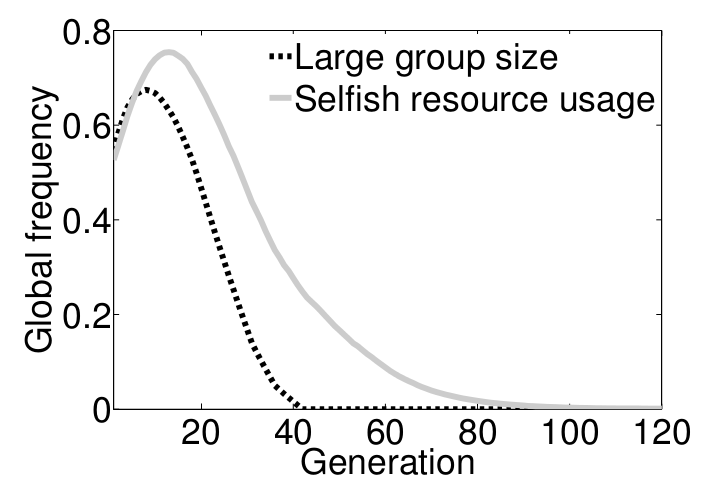
\includegraphics[width=0.4\textwidth]{orig_a.png}
                \caption{The original results from \cite{powers2007individual}.}
                \label{fig:orig:A}
        \end{subfigure}%
        ~ %add desired spacing between images, e. g. ~, \quad, \qquad etc.
          %(or a blank line to force the subfigure onto a new line)
        \begin{subfigure}[b]{0.4\textwidth}
                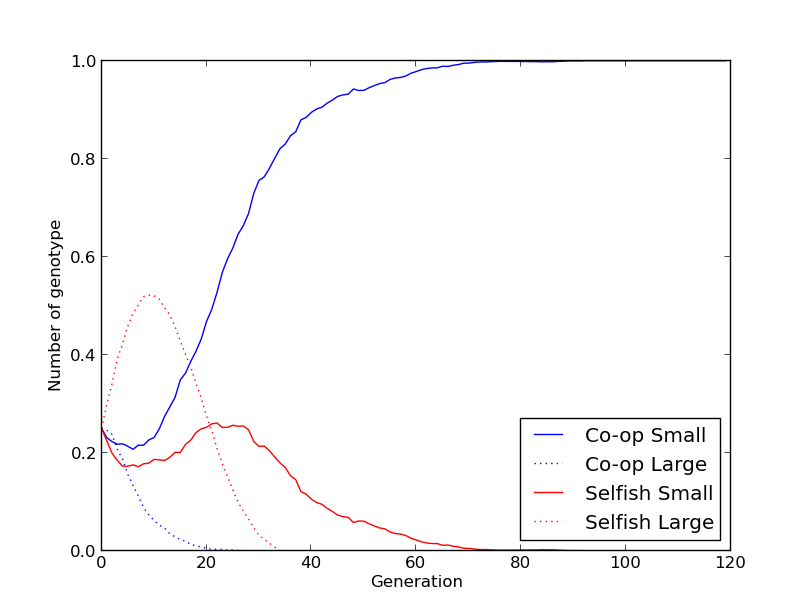
\includegraphics[width=0.4\textwidth]{Code2/fig1.png}
                \caption{Reproduced results.}
                \label{fig:orig:B}
        \end{subfigure}
        \caption{Average environment and strategy through time.}\label{fig:A}
\end{figure}

\begin{figure}
        \centering
        \begin{subfigure}[b]{0.4\textwidth}
                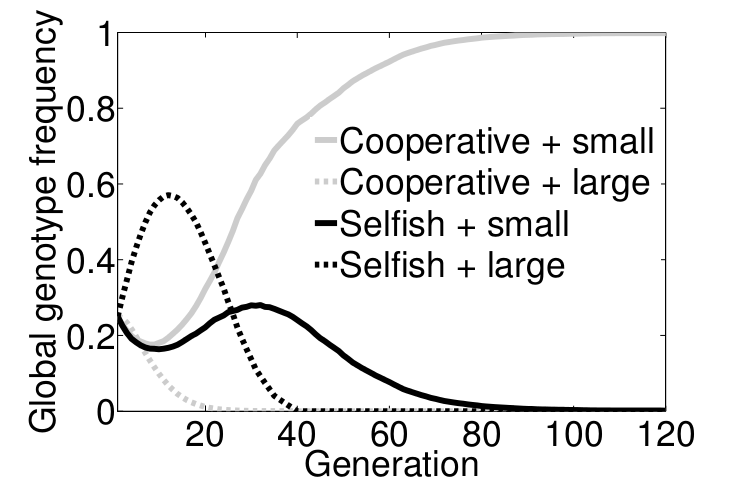
\includegraphics[width=\textwidth]{orig_b.png}
                \caption{The original results from \cite{powers2007individual}.}
                \label{fig:rep:A}
        \end{subfigure}%
        ~ %add desired spacing between images, e. g. ~, \quad, \qquad etc.
          %(or a blank line to force the subfigure onto a new line)
        \begin{subfigure}[b]{0.4\textwidth}
                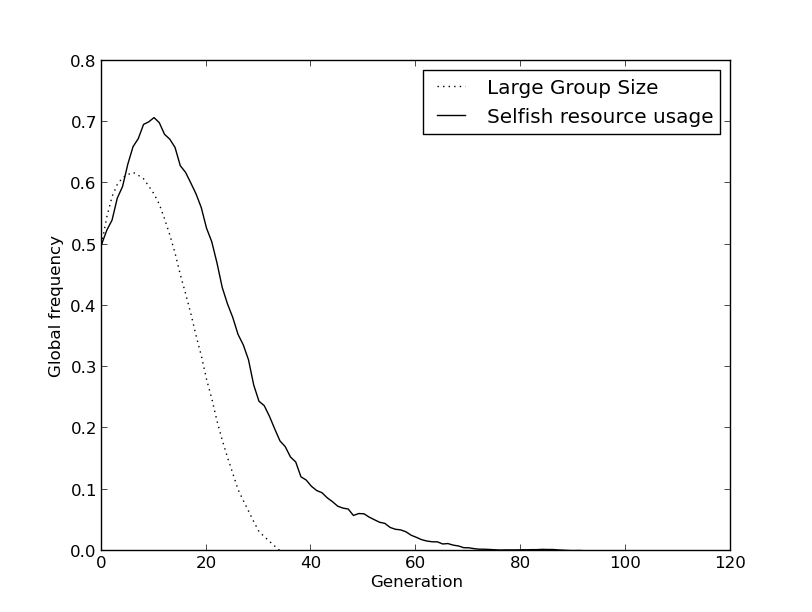
\includegraphics[width=\textwidth]{Code2/fig2.png}
                \caption{Reproduced results.}
                \label{fig:rep:B}
        \end{subfigure}
        \caption{Change in genotype frequencies over time.}\label{fig:B}
\end{figure}

The reproduced results were found to be very close to the original data. 
Figure \ref{fig:B} shows the proportion of each genotype in the population.
In both graphs, the cooperators in the large group get immediately out competed by the selfish, and are then pushed to extinction.
The numbers of large selfish then begin to diminish and both small genotypes increase before the cooperative small genotype excells and results in being the entire of the population.
The population reached a steady state by 100 generations.

Figure \ref{fig:A} shows the proportions of the strategies. 
Both results show that the large populations reach 0 first and the selfish gene takes a little longer to be removed from the population.

The results obtained from the extension proved to be a very close replication to the original data, and therefore can be used for an extension of this work.

\section{Extension}\label{sc:extension}

Discrete groups do not always occur in nature.
The extension covered here adds a third middle group to the experiment. 
The middle group contains all genotypes in the pool in the same proportions.
As before, an individual may only exist in one group. 
If it is in a middle group, then it cannot be in a small or large group.

The main parameters remain unchanged (apart from the number of generations, which was incresed to 200) from \cite{powers2007individual}.
This experiment set out to find when, if at all, the small cooperators were out competed by another genotype.
It is predicted that the large selfish genotype will take advantage of this middle group once a large enough proporiton of the population is placed in this.

NEED TO CITE SOME STUFF.



%why I am doing this extension

%my parameters
Some extra parameters were added to characterise the middle group. 
The size of this group, and the resources allocated, was made to be the average of the small and large group's size and resources. 
This was done to keep the same amount of resource per captia in the group.
The final parameter was the parameter under test - the proportion of the population that was placed in the medium sized group.
The parameters are summarised in table \ref{table:extparams}. 

\begin{table}
 \caption{The extra parameters used to implement the extension}
 \label{table:extparams}
 \begin{tabular}{|c|c|}
  Parameter, $symbol$ & value \\ \hline 
  Proportion of population in middle group, $M_{proportion}$ & $0.0 - 0.24$ \\ 
  Medium group size, $N_{med}$ & $22$ \\
  Medium group resource, $R_{med}$ & $27$ \\ \hline
 \end{tabular}
\end{table}


\section{Results}\label{sc:results}

A sweep of the middle proportions was done from $0$ to $0.24$. 
At each value of $M_{proportion}$, the simulation was run 10 times.
After each simulation, the genotype with the largest population was deemed to be the `winner' and a tally was kept. 
The number of wins of each genotype was plotted against the value of $M_{proportion}$ and can be seen in figure \ref{fig:extresult}.

The results show that the small cooperators win consistently until around $0.03$. 
From this point, the selfish large genotype starts to win some of the simulations. 
By $0.06$, large selfish starts to win the majority of the simulations.

Both small groups win the occasional game in the higher proportions. 
This is assumed to be noise as no explicit checking was done to verify the populations had reached fixation. 

\begin{figure}
 \centering
 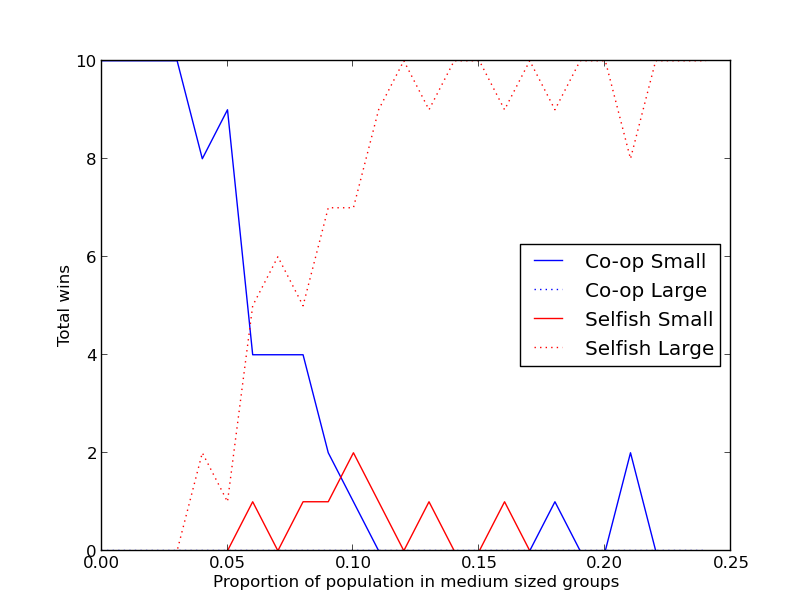
\includegraphics{Code2/extresults.png}
 \caption{A sweep of the proportion of the population allocated into medium sized groups.}
 \label{fig:extresult}
\end{figure}


\section{Conclusion}\label{sc:conclusion}

What I have done

What I have shown

Further work - make it continuous
However, this work still discretises the groups. Future work could improve this to have more groups, or even implement groups of many different sizes.
\bibliographystyle{apalike}
\bibliography{bibliography}
 
 \lstdefinelanguage{Python}{
 keywords={typeof, null, catch, switch, in, int, str, float, self},
 keywordstyle=\color{ForestGreen}\bfseries,
 ndkeywords={boolean, throw, import},
 ndkeywords={return, class, if ,elif, endif, while, do, else, True, False , catch, def},
 ndkeywordstyle=\color{BrickRed}\bfseries,
 identifierstyle=\color{black},
 sensitive=false,
 comment=[l]{\#},
 morecomment=[s]{/*}{*/},
 commentstyle=\color{purple}\ttfamily,
 stringstyle=\color{red}\ttfamily,
}

 \clearpage
 \section{Code}
 \lstset{language=Python} 
 \subsection{main.py}
 \lstinputlisting[language=Python,caption=Reimplementation of \cite{powers2007individual}]{Code2/main.py}

\end{document}
